% Generated by make_fig_b_example.py. Do not edit by hand.
\documentclass[tikz,border=1pt]{standalone}
\usepackage[T1]{fontenc}
\usepackage{newtxtext,newtxmath}
\usepackage[varqu,scaled=0.95]{zi4}
\usetikzlibrary{positioning}
\definecolor{ink}{HTML}{1F2328}\definecolor{mute}{HTML}{6E7781}
\definecolor{wire}{HTML}{24527F}\definecolor{qbg}{HTML}{DCE7F3}\definecolor{cbg}{HTML}{EEF0F2}
\definecolor{kw}{HTML}{24527F}\definecolor{str}{HTML}{8A4B08}
\tikzset{
  code/.style={anchor=base west, inner sep=0pt, font=\ttfamily\fontsize{8}{9.6}\selectfont, text=ink},
  num/.style={anchor=base east, inner sep=0pt, font=\ttfamily\fontsize{7}{9.6}\selectfont, text=mute},
  hdr/.style={anchor=base, inner sep=0pt, font=\fontsize{7}{8}\selectfont, text=ink, align=center},
  key/.style={anchor=base west, inner sep=0pt, font=\fontsize{7}{8}\selectfont, text=ink},
}
\begin{document}
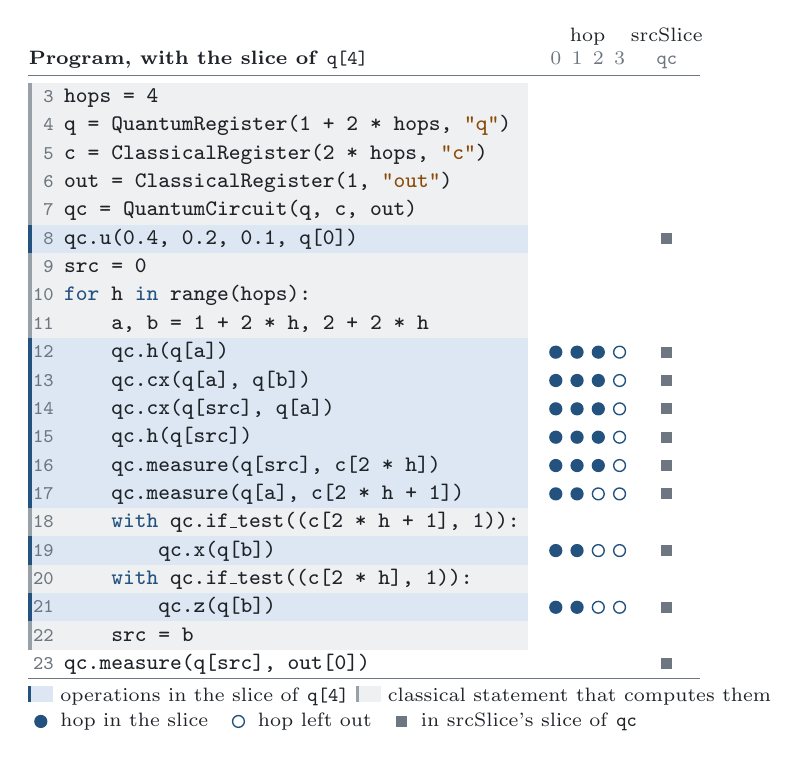
\begin{tikzpicture}

\node[hdr] at (6.655,0.42) {hop};
\node[hdr, text=mute] at (6.25,0.12) {0};
\node[hdr, text=mute] at (6.52,0.12) {1};
\node[hdr, text=mute] at (6.79,0.12) {2};
\node[hdr, text=mute] at (7.0600000000000005,0.12) {3};
\node[hdr, anchor=base west] at (-0.45,0.12) {\bfseries Program, with the slice of \texttt{q[4]}};
\node[hdr] at (7.66,0.42) {srcSlice};
\node[hdr, text=mute] at (7.66,0.12) {\texttt{qc}};
\draw[mute, line width=0.4pt] (-0.45,-0.02) -- (8.08,-0.02);
\fill[cbg] (-0.45,-0.470) rectangle (5.9,-0.110);
\fill[mute!70] (-0.45,-0.470) rectangle (-0.4,-0.110);
\node[num] at (-0.12,-0.360) {3};
\node[code] at (0.0,-0.360) {hops\ =\ 4};
\fill[cbg] (-0.45,-0.830) rectangle (5.9,-0.470);
\fill[mute!70] (-0.45,-0.830) rectangle (-0.4,-0.470);
\node[num] at (-0.12,-0.720) {4};
\node[code] at (0.0,-0.720) {q\ =\ QuantumRegister(1\ +\ 2\ *\ hops,\ \textcolor{str}{"q"})};
\fill[cbg] (-0.45,-1.190) rectangle (5.9,-0.830);
\fill[mute!70] (-0.45,-1.190) rectangle (-0.4,-0.830);
\node[num] at (-0.12,-1.080) {5};
\node[code] at (0.0,-1.080) {c\ =\ ClassicalRegister(2\ *\ hops,\ \textcolor{str}{"c"})};
\fill[cbg] (-0.45,-1.550) rectangle (5.9,-1.190);
\fill[mute!70] (-0.45,-1.550) rectangle (-0.4,-1.190);
\node[num] at (-0.12,-1.440) {6};
\node[code] at (0.0,-1.440) {out\ =\ ClassicalRegister(1,\ \textcolor{str}{"out"})};
\fill[cbg] (-0.45,-1.910) rectangle (5.9,-1.550);
\fill[mute!70] (-0.45,-1.910) rectangle (-0.4,-1.550);
\node[num] at (-0.12,-1.800) {7};
\node[code] at (0.0,-1.800) {qc\ =\ QuantumCircuit(q,\ c,\ out)};
\fill[qbg] (-0.45,-2.270) rectangle (5.9,-1.910);
\fill[wire] (-0.45,-2.270) rectangle (-0.4,-1.910);
\node[num] at (-0.12,-2.160) {8};
\node[code] at (0.0,-2.160) {qc.u(0.4,\ 0.2,\ 0.1,\ q[0])};
\fill[mute] (7.59,-2.16) rectangle ++(0.14,0.14);
\fill[cbg] (-0.45,-2.630) rectangle (5.9,-2.270);
\fill[mute!70] (-0.45,-2.630) rectangle (-0.4,-2.270);
\node[num] at (-0.12,-2.520) {9};
\node[code] at (0.0,-2.520) {src\ =\ 0};
\fill[cbg] (-0.45,-2.990) rectangle (5.9,-2.630);
\fill[mute!70] (-0.45,-2.990) rectangle (-0.4,-2.630);
\node[num] at (-0.12,-2.880) {10};
\node[code] at (0.0,-2.880) {\textcolor{kw}{\bfseries for}\ h\ \textcolor{kw}{\bfseries in}\ range(hops):};
\fill[cbg] (-0.45,-3.350) rectangle (5.9,-2.990);
\fill[mute!70] (-0.45,-3.350) rectangle (-0.4,-2.990);
\node[num] at (-0.12,-3.240) {11};
\node[code] at (0.0,-3.240) {\ \ \ \ a,\ b\ =\ 1\ +\ 2\ *\ h,\ 2\ +\ 2\ *\ h};
\fill[qbg] (-0.45,-3.710) rectangle (5.9,-3.350);
\fill[wire] (-0.45,-3.710) rectangle (-0.4,-3.350);
\node[num] at (-0.12,-3.600) {12};
\node[code] at (0.0,-3.600) {\ \ \ \ qc.h(q[a])};
\draw[wire, line width=0.5pt, fill=wire] (6.25,-3.530) circle (0.075);
\draw[wire, line width=0.5pt, fill=wire] (6.52,-3.530) circle (0.075);
\draw[wire, line width=0.5pt, fill=wire] (6.79,-3.530) circle (0.075);
\draw[wire, line width=0.5pt, fill=white] (7.0600000000000005,-3.530) circle (0.075);
\fill[mute] (7.59,-3.5999999999999996) rectangle ++(0.14,0.14);
\fill[qbg] (-0.45,-4.070) rectangle (5.9,-3.710);
\fill[wire] (-0.45,-4.070) rectangle (-0.4,-3.710);
\node[num] at (-0.12,-3.960) {13};
\node[code] at (0.0,-3.960) {\ \ \ \ qc.cx(q[a],\ q[b])};
\draw[wire, line width=0.5pt, fill=wire] (6.25,-3.890) circle (0.075);
\draw[wire, line width=0.5pt, fill=wire] (6.52,-3.890) circle (0.075);
\draw[wire, line width=0.5pt, fill=wire] (6.79,-3.890) circle (0.075);
\draw[wire, line width=0.5pt, fill=white] (7.0600000000000005,-3.890) circle (0.075);
\fill[mute] (7.59,-3.96) rectangle ++(0.14,0.14);
\fill[qbg] (-0.45,-4.430) rectangle (5.9,-4.070);
\fill[wire] (-0.45,-4.430) rectangle (-0.4,-4.070);
\node[num] at (-0.12,-4.320) {14};
\node[code] at (0.0,-4.320) {\ \ \ \ qc.cx(q[src],\ q[a])};
\draw[wire, line width=0.5pt, fill=wire] (6.25,-4.250) circle (0.075);
\draw[wire, line width=0.5pt, fill=wire] (6.52,-4.250) circle (0.075);
\draw[wire, line width=0.5pt, fill=wire] (6.79,-4.250) circle (0.075);
\draw[wire, line width=0.5pt, fill=white] (7.0600000000000005,-4.250) circle (0.075);
\fill[mute] (7.59,-4.32) rectangle ++(0.14,0.14);
\fill[qbg] (-0.45,-4.790) rectangle (5.9,-4.430);
\fill[wire] (-0.45,-4.790) rectangle (-0.4,-4.430);
\node[num] at (-0.12,-4.680) {15};
\node[code] at (0.0,-4.680) {\ \ \ \ qc.h(q[src])};
\draw[wire, line width=0.5pt, fill=wire] (6.25,-4.610) circle (0.075);
\draw[wire, line width=0.5pt, fill=wire] (6.52,-4.610) circle (0.075);
\draw[wire, line width=0.5pt, fill=wire] (6.79,-4.610) circle (0.075);
\draw[wire, line width=0.5pt, fill=white] (7.0600000000000005,-4.610) circle (0.075);
\fill[mute] (7.59,-4.68) rectangle ++(0.14,0.14);
\fill[qbg] (-0.45,-5.150) rectangle (5.9,-4.790);
\fill[wire] (-0.45,-5.150) rectangle (-0.4,-4.790);
\node[num] at (-0.12,-5.040) {16};
\node[code] at (0.0,-5.040) {\ \ \ \ qc.measure(q[src],\ c[2\ *\ h])};
\draw[wire, line width=0.5pt, fill=wire] (6.25,-4.970) circle (0.075);
\draw[wire, line width=0.5pt, fill=wire] (6.52,-4.970) circle (0.075);
\draw[wire, line width=0.5pt, fill=wire] (6.79,-4.970) circle (0.075);
\draw[wire, line width=0.5pt, fill=white] (7.0600000000000005,-4.970) circle (0.075);
\fill[mute] (7.59,-5.04) rectangle ++(0.14,0.14);
\fill[qbg] (-0.45,-5.510) rectangle (5.9,-5.150);
\fill[wire] (-0.45,-5.510) rectangle (-0.4,-5.150);
\node[num] at (-0.12,-5.400) {17};
\node[code] at (0.0,-5.400) {\ \ \ \ qc.measure(q[a],\ c[2\ *\ h\ +\ 1])};
\draw[wire, line width=0.5pt, fill=wire] (6.25,-5.330) circle (0.075);
\draw[wire, line width=0.5pt, fill=wire] (6.52,-5.330) circle (0.075);
\draw[wire, line width=0.5pt, fill=white] (6.79,-5.330) circle (0.075);
\draw[wire, line width=0.5pt, fill=white] (7.0600000000000005,-5.330) circle (0.075);
\fill[mute] (7.59,-5.3999999999999995) rectangle ++(0.14,0.14);
\fill[cbg] (-0.45,-5.870) rectangle (5.9,-5.510);
\fill[mute!70] (-0.45,-5.870) rectangle (-0.4,-5.510);
\node[num] at (-0.12,-5.760) {18};
\node[code] at (0.0,-5.760) {\ \ \ \ \textcolor{kw}{\bfseries with}\ qc.if\_test((c[2\ *\ h\ +\ 1],\ 1)):};
\fill[qbg] (-0.45,-6.230) rectangle (5.9,-5.870);
\fill[wire] (-0.45,-6.230) rectangle (-0.4,-5.870);
\node[num] at (-0.12,-6.120) {19};
\node[code] at (0.0,-6.120) {\ \ \ \ \ \ \ \ qc.x(q[b])};
\draw[wire, line width=0.5pt, fill=wire] (6.25,-6.050) circle (0.075);
\draw[wire, line width=0.5pt, fill=wire] (6.52,-6.050) circle (0.075);
\draw[wire, line width=0.5pt, fill=white] (6.79,-6.050) circle (0.075);
\draw[wire, line width=0.5pt, fill=white] (7.0600000000000005,-6.050) circle (0.075);
\fill[mute] (7.59,-6.12) rectangle ++(0.14,0.14);
\fill[cbg] (-0.45,-6.590) rectangle (5.9,-6.230);
\fill[mute!70] (-0.45,-6.590) rectangle (-0.4,-6.230);
\node[num] at (-0.12,-6.480) {20};
\node[code] at (0.0,-6.480) {\ \ \ \ \textcolor{kw}{\bfseries with}\ qc.if\_test((c[2\ *\ h],\ 1)):};
\fill[qbg] (-0.45,-6.950) rectangle (5.9,-6.590);
\fill[wire] (-0.45,-6.950) rectangle (-0.4,-6.590);
\node[num] at (-0.12,-6.840) {21};
\node[code] at (0.0,-6.840) {\ \ \ \ \ \ \ \ qc.z(q[b])};
\draw[wire, line width=0.5pt, fill=wire] (6.25,-6.770) circle (0.075);
\draw[wire, line width=0.5pt, fill=wire] (6.52,-6.770) circle (0.075);
\draw[wire, line width=0.5pt, fill=white] (6.79,-6.770) circle (0.075);
\draw[wire, line width=0.5pt, fill=white] (7.0600000000000005,-6.770) circle (0.075);
\fill[mute] (7.59,-6.84) rectangle ++(0.14,0.14);
\fill[cbg] (-0.45,-7.310) rectangle (5.9,-6.950);
\fill[mute!70] (-0.45,-7.310) rectangle (-0.4,-6.950);
\node[num] at (-0.12,-7.200) {22};
\node[code] at (0.0,-7.200) {\ \ \ \ src\ =\ b};
\node[num] at (-0.12,-7.560) {23};
\node[code] at (0.0,-7.560) {qc.measure(q[src],\ out[0])};
\fill[mute] (7.59,-7.56) rectangle ++(0.14,0.14);
\draw[mute, line width=0.4pt] (-0.45,-7.670) -- (8.08,-7.670);
\begin{scope}[shift={(-0.45,-7.970)}] \fill[qbg] (0,0) rectangle (0.32,0.2); \fill[wire] (0,0) rectangle (0.04,0.2); \end{scope}
\node[key] (k) at (-0.04999999999999999,-7.970) {operations in the slice of \texttt{q[4]}};
\begin{scope}[shift={(3.71,-7.970)}] \fill[cbg] (0,0) rectangle (0.32,0.2); \fill[mute!70] (0,0) rectangle (0.04,0.2); \end{scope}
\node[key] (k) at (4.11,-7.970) {classical statement that computes them};
\begin{scope}[shift={(-0.45,-8.290)}] \draw[wire, line width=0.5pt, fill=wire] (0.16,0.07) circle (0.075); \end{scope}
\node[key] (k) at (-0.04999999999999999,-8.290) {hop in the slice};
\begin{scope}[shift={(2.06,-8.290)}] \draw[wire, line width=0.5pt, fill=white] (0.16,0.07) circle (0.075); \end{scope}
\node[key] (k) at (2.46,-8.290) {hop left out};
\begin{scope}[shift={(4.130000000000001,-8.290)}] \fill[mute] (0.09,0) rectangle ++(0.14,0.14); \end{scope}
\node[key] (k) at (4.530000000000001,-8.290) {in srcSlice's slice of \texttt{qc}};
\end{tikzpicture}
\end{document}
